\section{Preguntas}

\subsection{How is mesh size convergence determined?}

Mesh size convergence is achieved when further refinement of the mesh does not significantly alter the solution of the problem.  
This can be verified by comparing results such as displacements, Von Mises stresses, and principal stresses across different mesh sizes.  
In this case, convergence was assessed by plotting the maximum Von Mises stress against the characteristic length, while also observing the processing time for each mesh.  
The results show that at a characteristic length $L_c = 0.8$, the mesh had already reached convergence.

\begin{figure}[H]
    \centering
    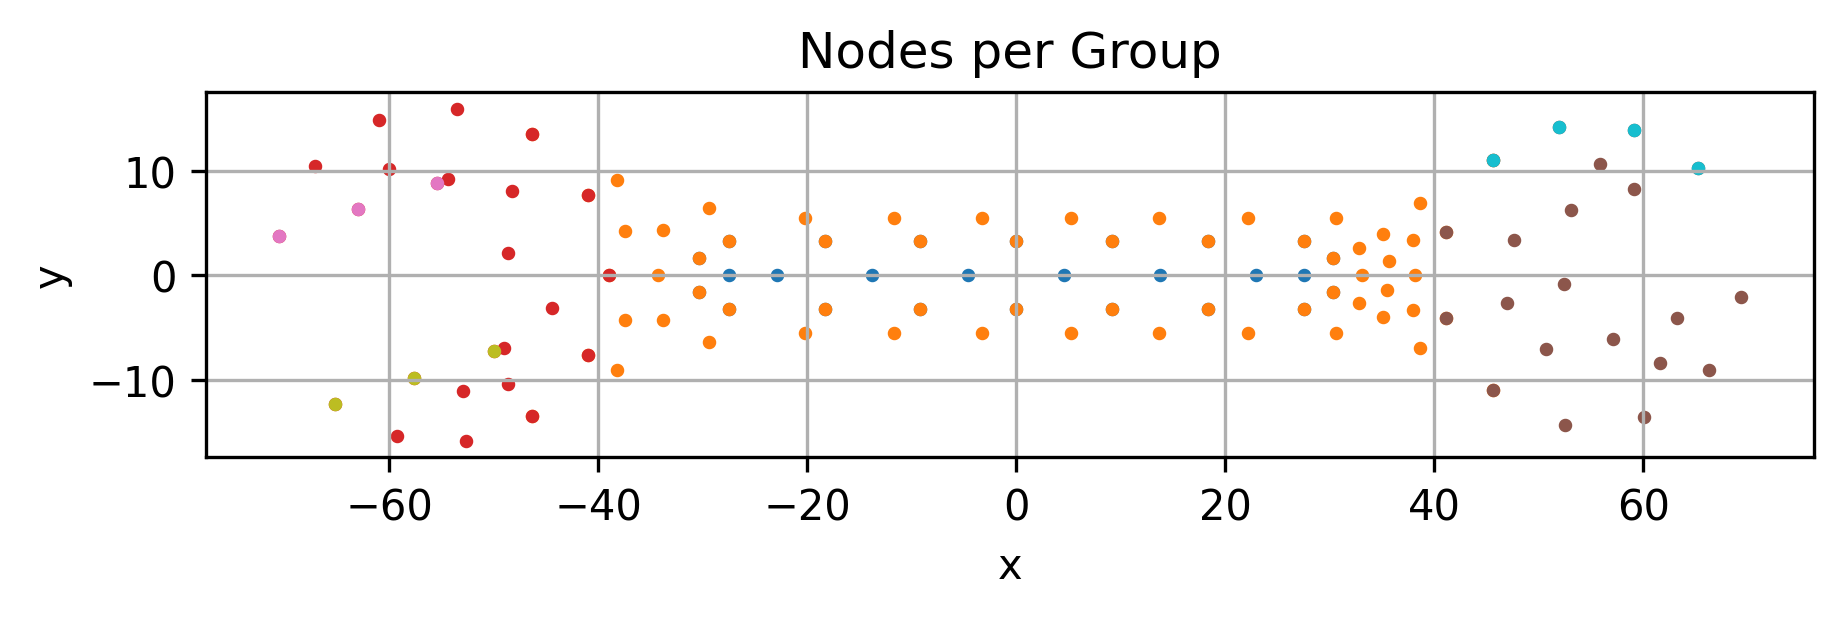
\includegraphics[width=0.8\textwidth]{GRAFICOS/Initial_nodes_por_grupo.png}
    \caption{Initial nodal distribution for the coarse mesh.}
    \label{fig:initial_nodes}
\end{figure}
  
\begin{figure}[H]
    \centering
    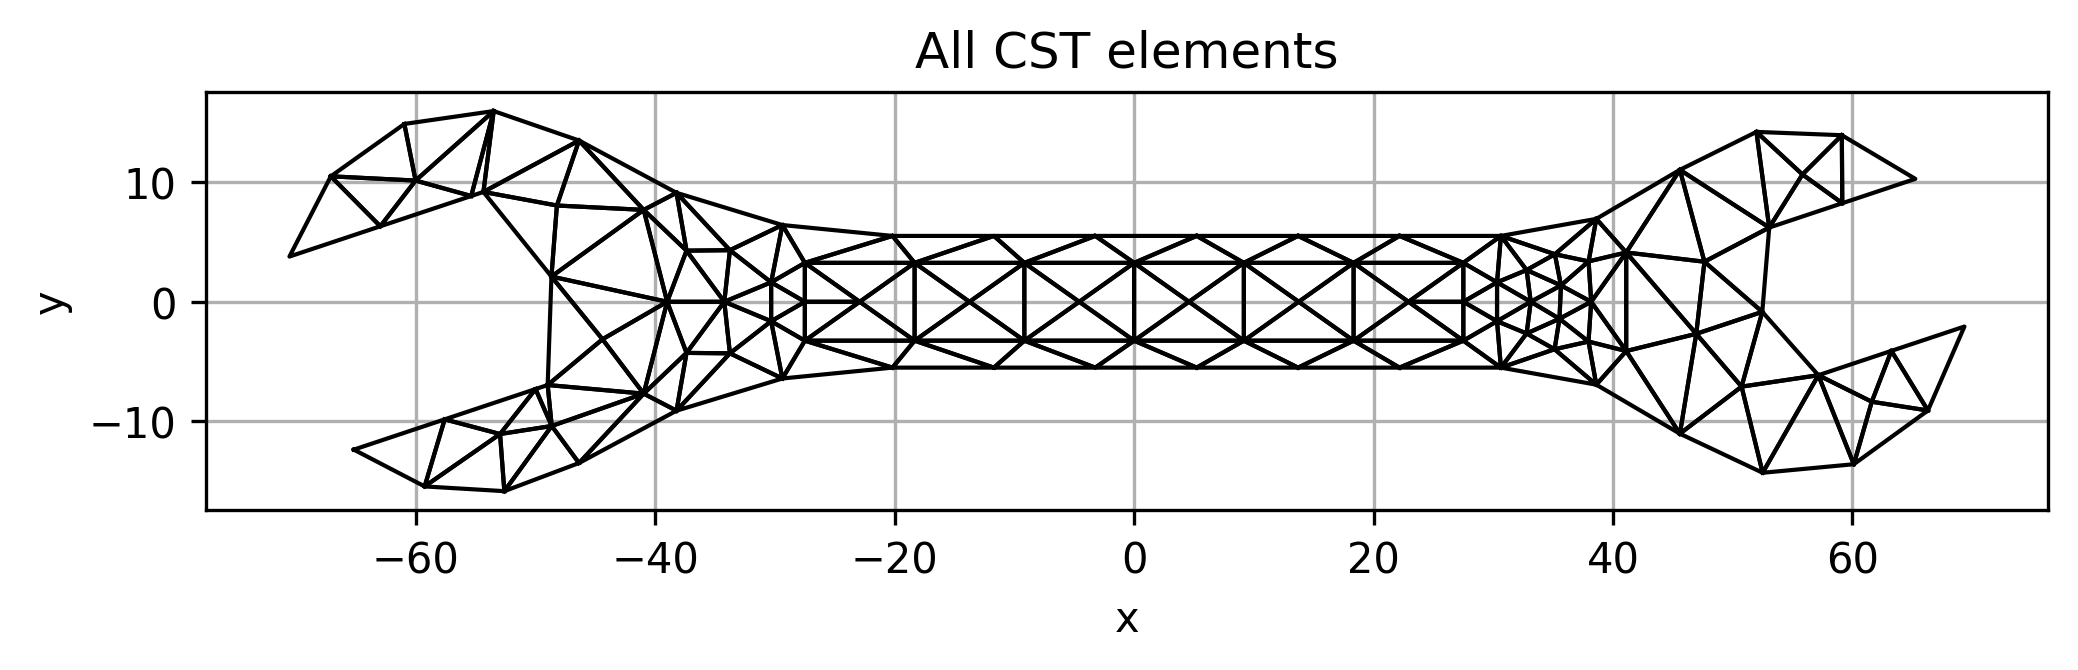
\includegraphics[width=0.8\textwidth]{GRAFICOS/Initial_elementos.png}
    \caption{Initial element distribution for the coarse mesh.}
    \label{fig:initial_elements}
\end{figure}
  
A script was developed to plot the convergence behavior of the mesh based on the execution time.

\begin{figure}[H]
    \centering
    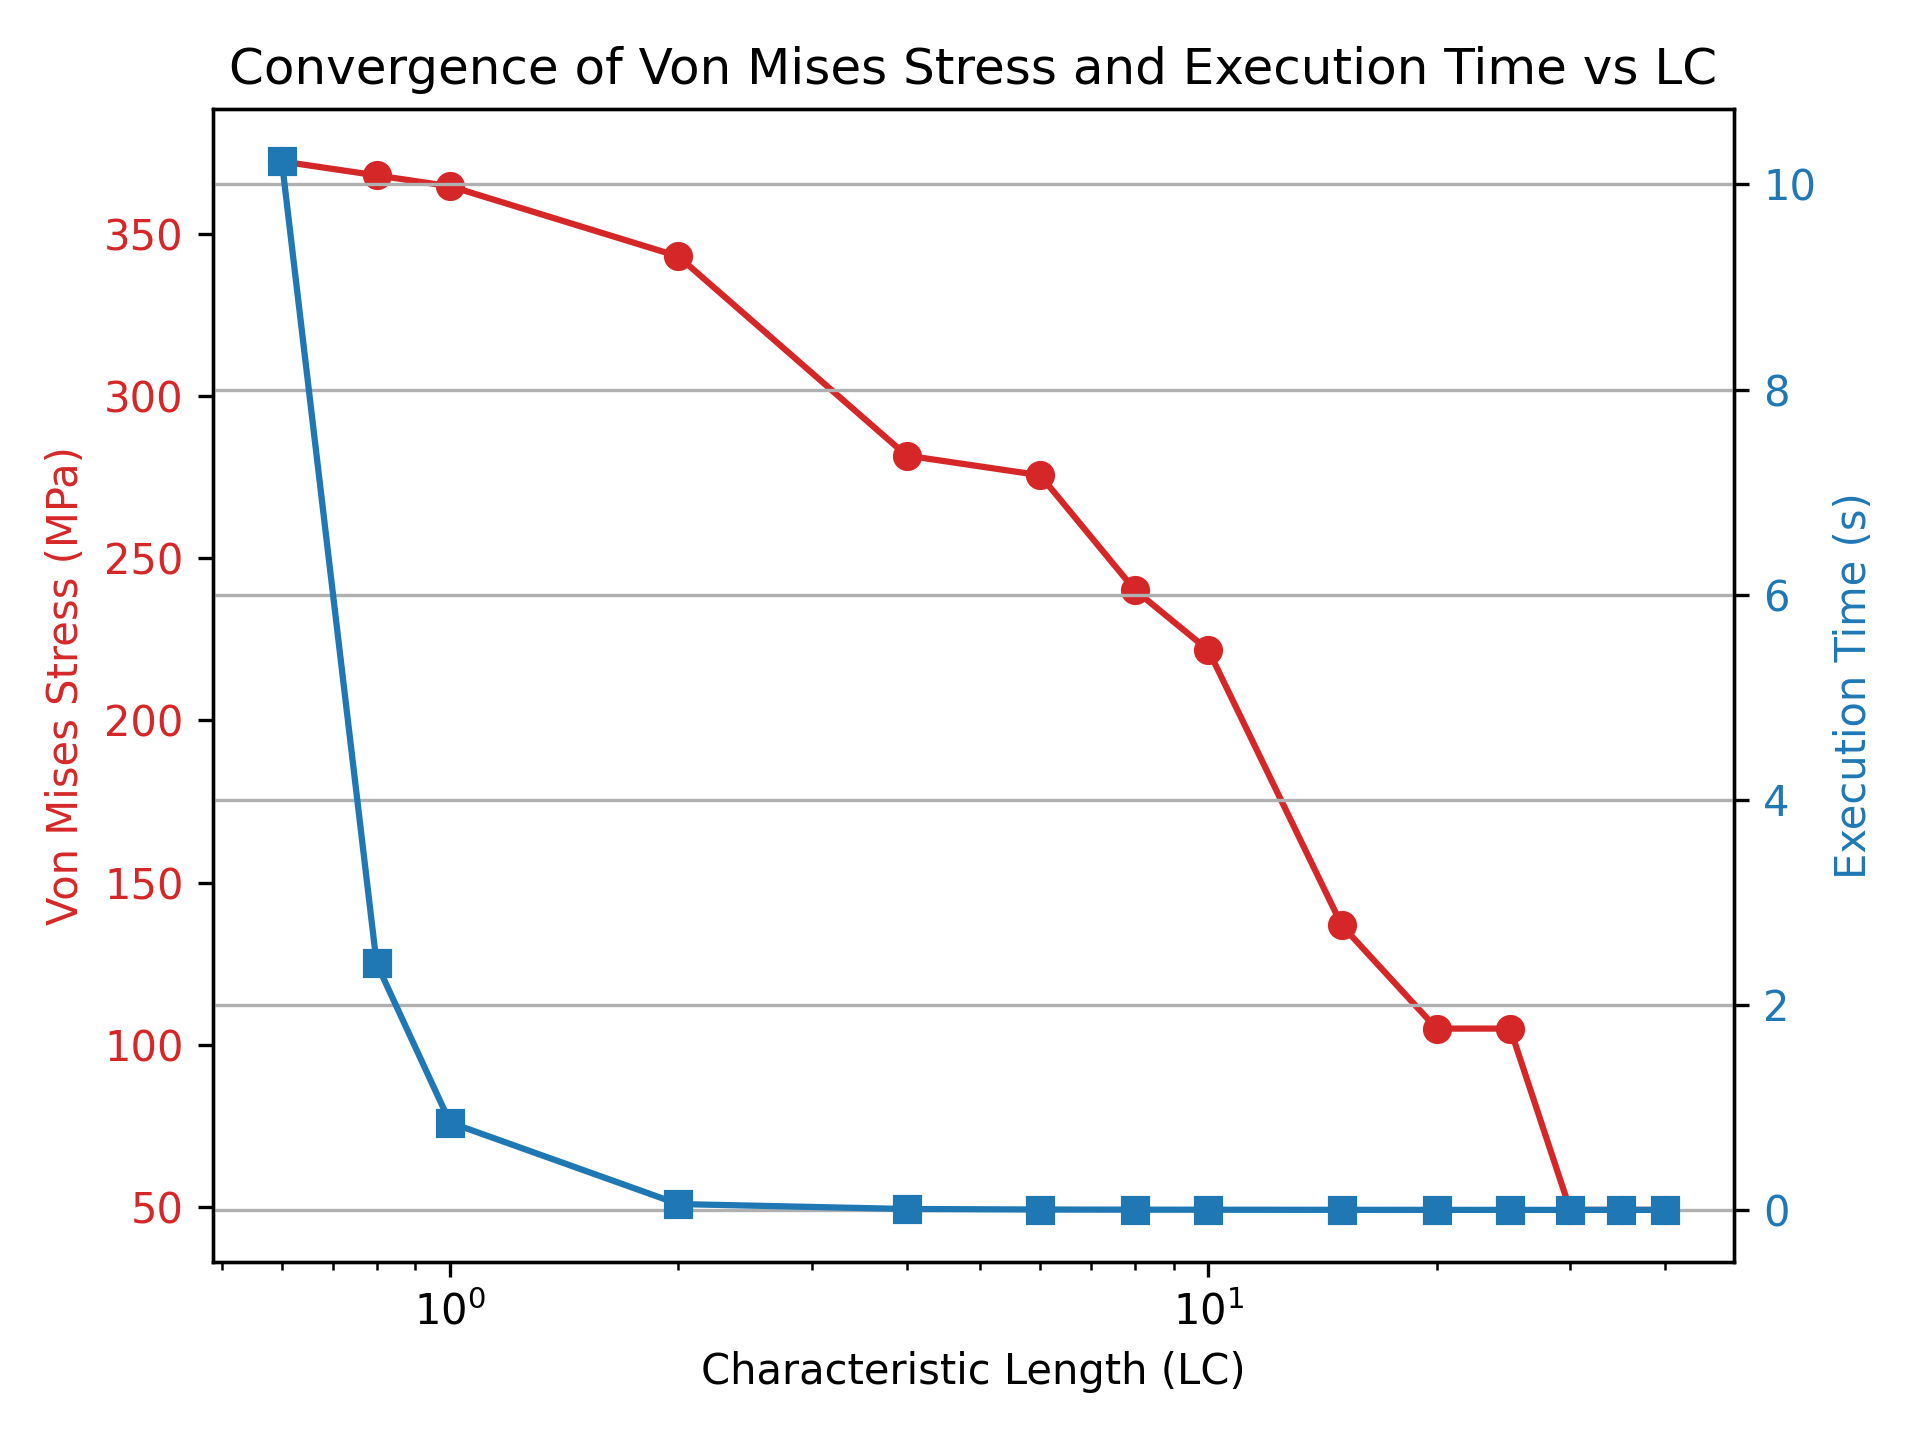
\includegraphics[width=0.6\textwidth]{GRAFICOS/convergence.png}
    \caption{Convergence curve: maximum Von Mises stress and execution time versus characteristic length.}
    \label{fig:convergence_curve}
\end{figure}

The result confirmed that $L_c = 0.8$ provides a good balance between computational cost and solution accuracy.

Therefore, the final model after mesh convergence is illustrated below:

\begin{figure}[H]
    \centering
    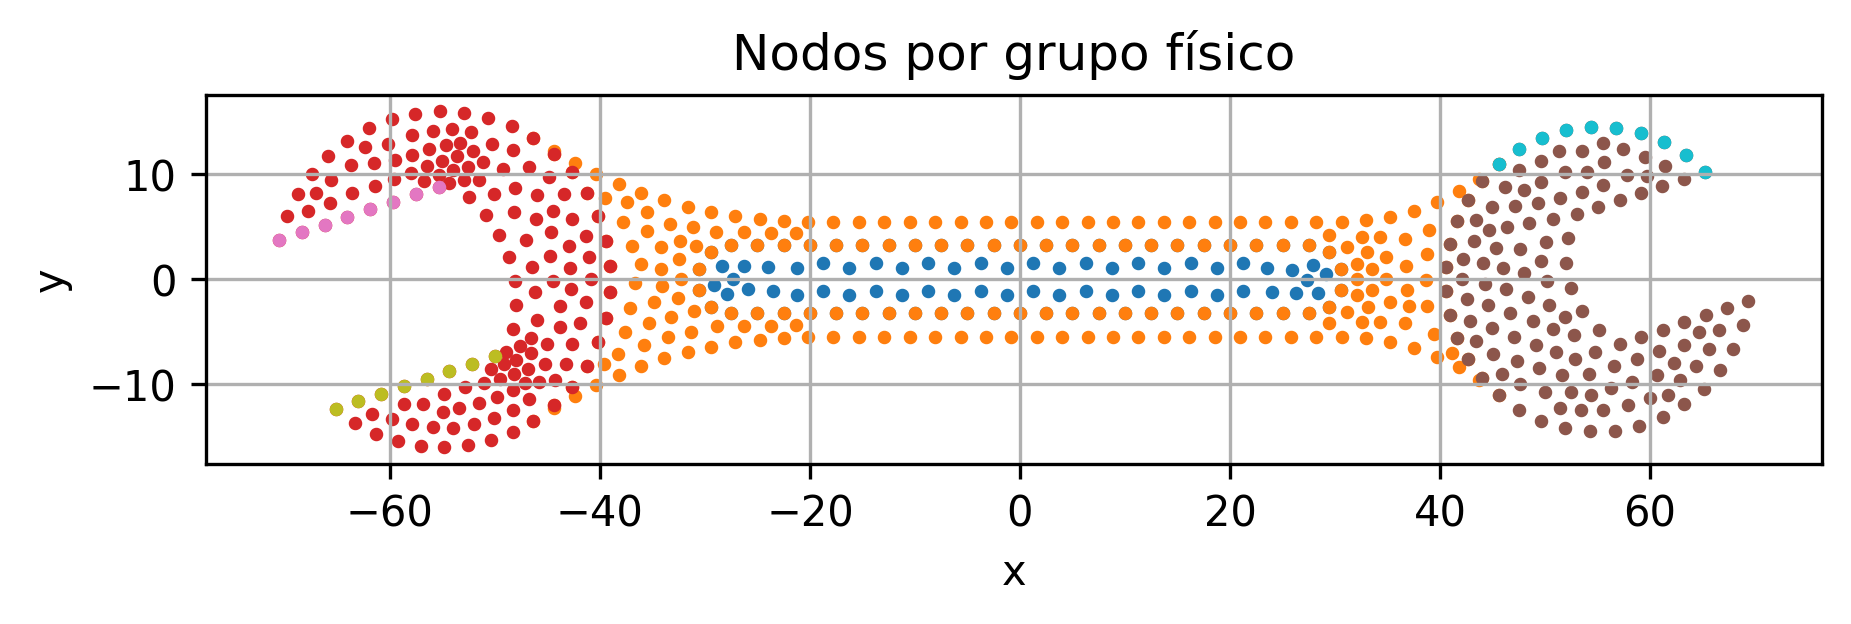
\includegraphics[width=0.8\textwidth]{GRAFICOS/Case a_nodes_por_grupo.png}
    \caption{Final nodal distribution after mesh convergence.}
    \label{fig:final_nodes}
\end{figure}
  
\begin{figure}[H]
    \centering
    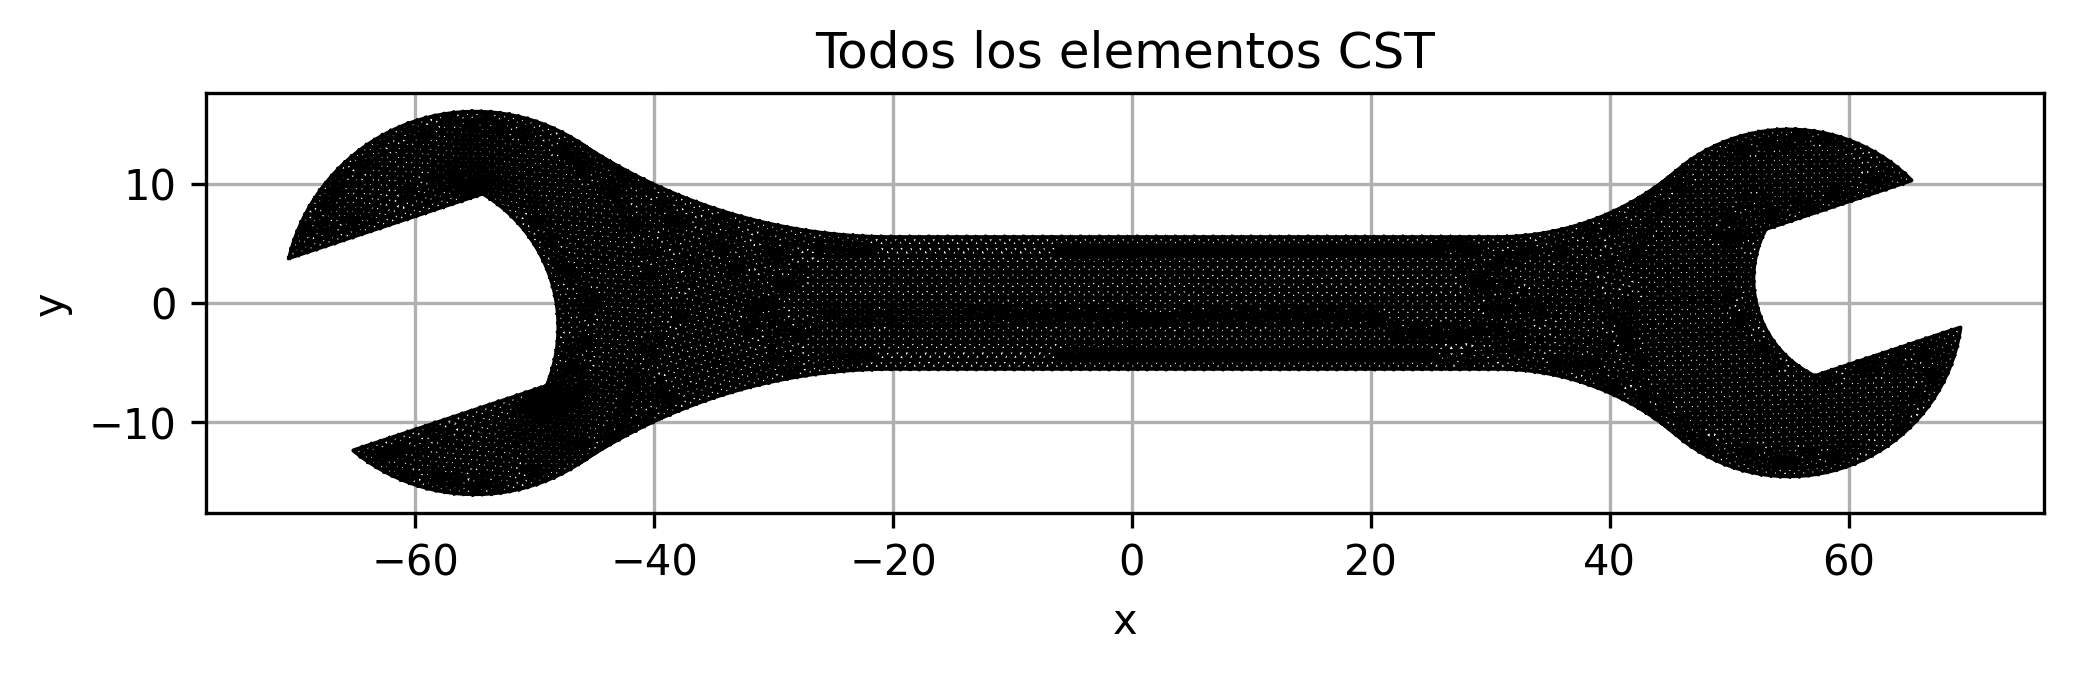
\includegraphics[width=0.8\textwidth]{GRAFICOS/Case a_elementos.png}
    \caption{Final element distribution after mesh convergence.}
    \label{fig:final_elements}
\end{figure}

\subsection{How do the stress/strain fields look like before and after smoothing?}

Before smoothing, the stress and strain fields shows abrubt jumps between adjacent elements (as sees in apendices section), producing a non-physical behaviour and dicontinuous fields. It is expected due to the implementation of CST elements, which have a constant stress and strain state. After applying post-processing smoothing, the fields becmoe continuous, whit better transitions across the domain, making it physically accurate.

\subsection{What differences do you observe when applying the load as a distributed load versus a point load?}

As a distributed load results in smoother and more realistic stress fiels, as the force is spread over an area, avoiding axcessive stress concentrations. 
On the other hand, a point load produces localized hight-stress peaks near the application point, leading to unrealistic stress values, unless the mesh is highly refined.

\subsection{Is it necessary to consider self-weight for an accurate analysis of the tool?}

In this case, it is not necessary to consider it, because the external forces applied are significantly grater than de self-weight of the PLA material. 
However, numercial comparisons showed that including self-weight, slightly increases the overall stress and displacement values, especially un ling or thin sections.

\subsection{Research or provide a reasonable stress-based failure criteria for PLA. For this loading condition, and based on
your failure criteria ¿where do you expect the wrench to fail?}

According to \citet{farah2016}, PLA (Polylactic Acid) exhibits a tensile strength near 50 MPa, depending on molecular weight, crystallinity, and processing method. Additionally, the usual Young's module is about 3.5 GPa, and the material has a relatively low elongation at break (about $4\text{-}7\%$), confirming its brittle nature.

Therefore, a reasonable stress-based failure criteria for PLA under mechanical loading is the Von Mises yield criterion, assuming brittle fracture at an equivalent stress level of around 50 MPa. Given PLA's limited ductility and tendency to fail without significant plastic deformation, reaching the ultimate tensile strength would iniciate cracking or brittle rupture.

As a result, based on the FEM simulations and stress distribution results, the highest Von Mises stresses concentrated at the junction between the wrench handle and the wrench head would be an expected failure location, in other words, near sharp geometrical transitions or areas under bending moments.

\subsection{Topological Optimization}

In order to reduce peak stress concentrations, a topological optimization was implemented based on the von Mises stress field. Elements with higher von Mises stress values had their thickness increased, while elements with lower von Mises stress values had their thickness reduced.  
To maintain the overall weight of the structure, several iterations were performed until the final model was obtained.  
The results are shown in the following figures:

\begin{figure}[H]
    \centering
    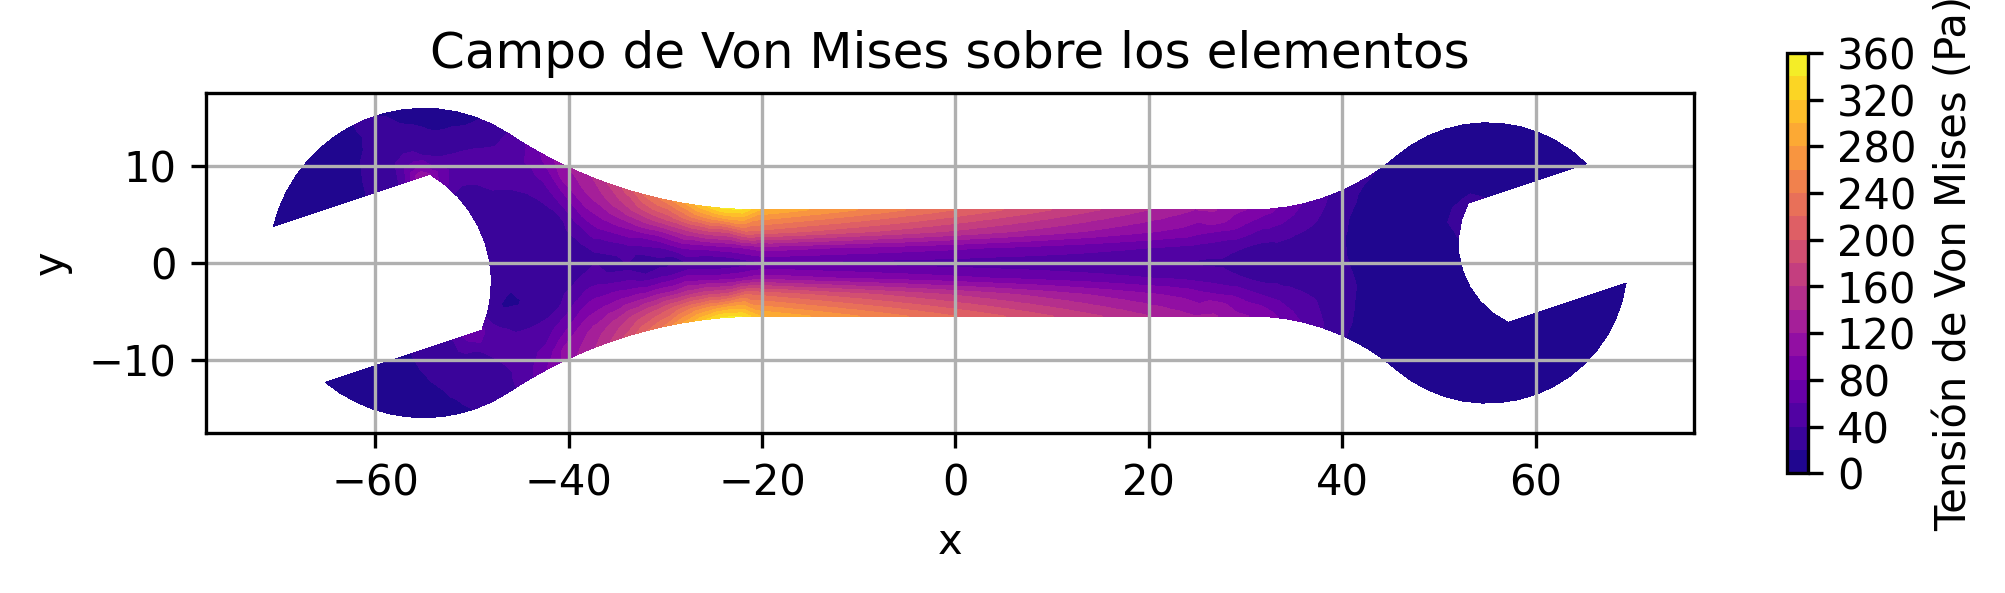
\includegraphics[width=0.8\textwidth]{GRAFICOS/Topo_ini_von_mises.png}
    \caption{Von Mises stress distribution before optimization.}
    \label{fig:von_mises_initial}
\end{figure}

\begin{figure}[H]
    \centering
    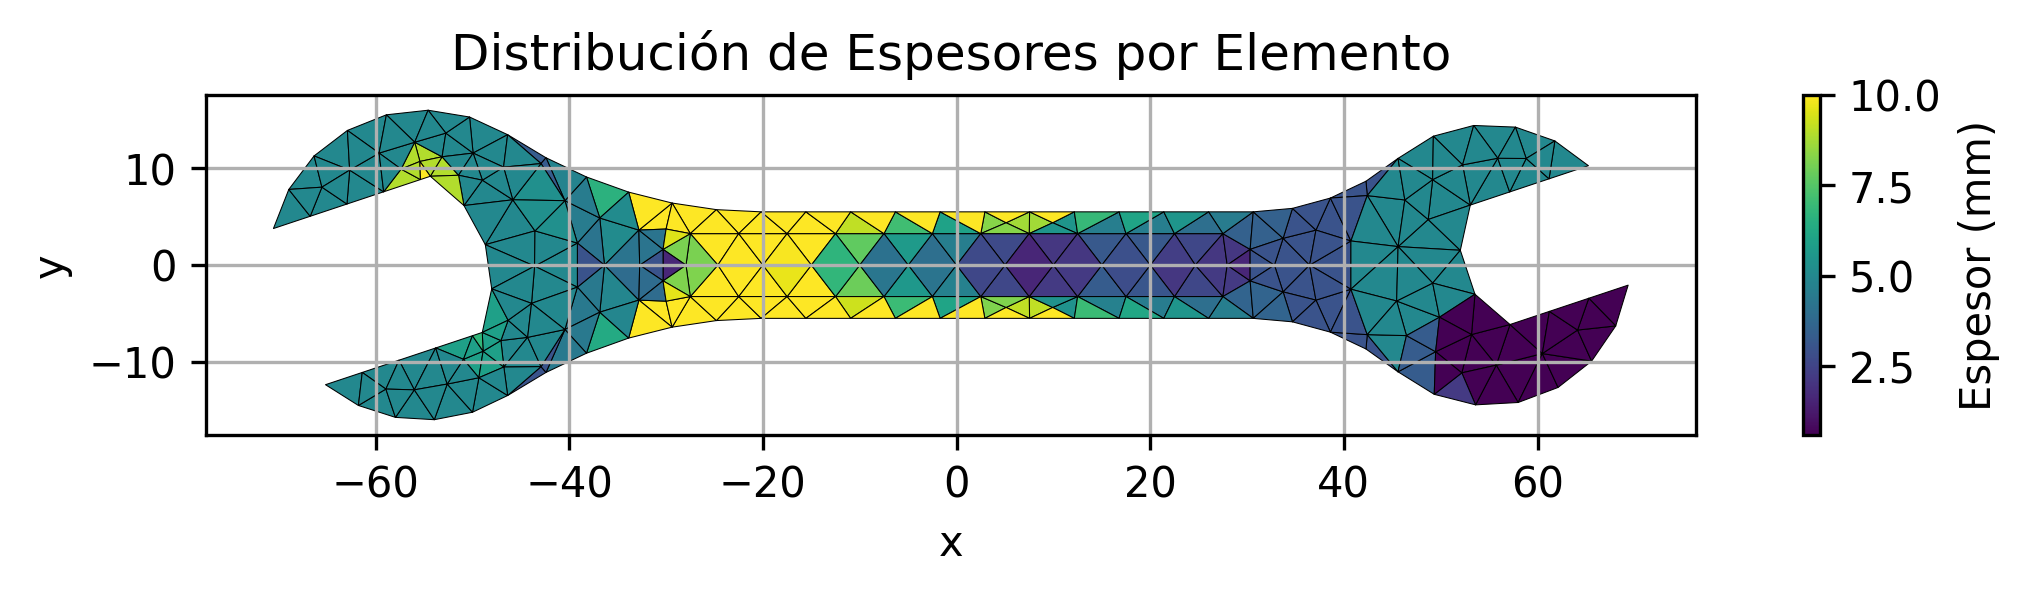
\includegraphics[width=0.8\textwidth]{GRAFICOS/espesores_espesores.png}
    \caption{Final thickness distribution after optimization.}
    \label{fig:thickness_distribution}
\end{figure}

\begin{figure}[H]
    \centering
    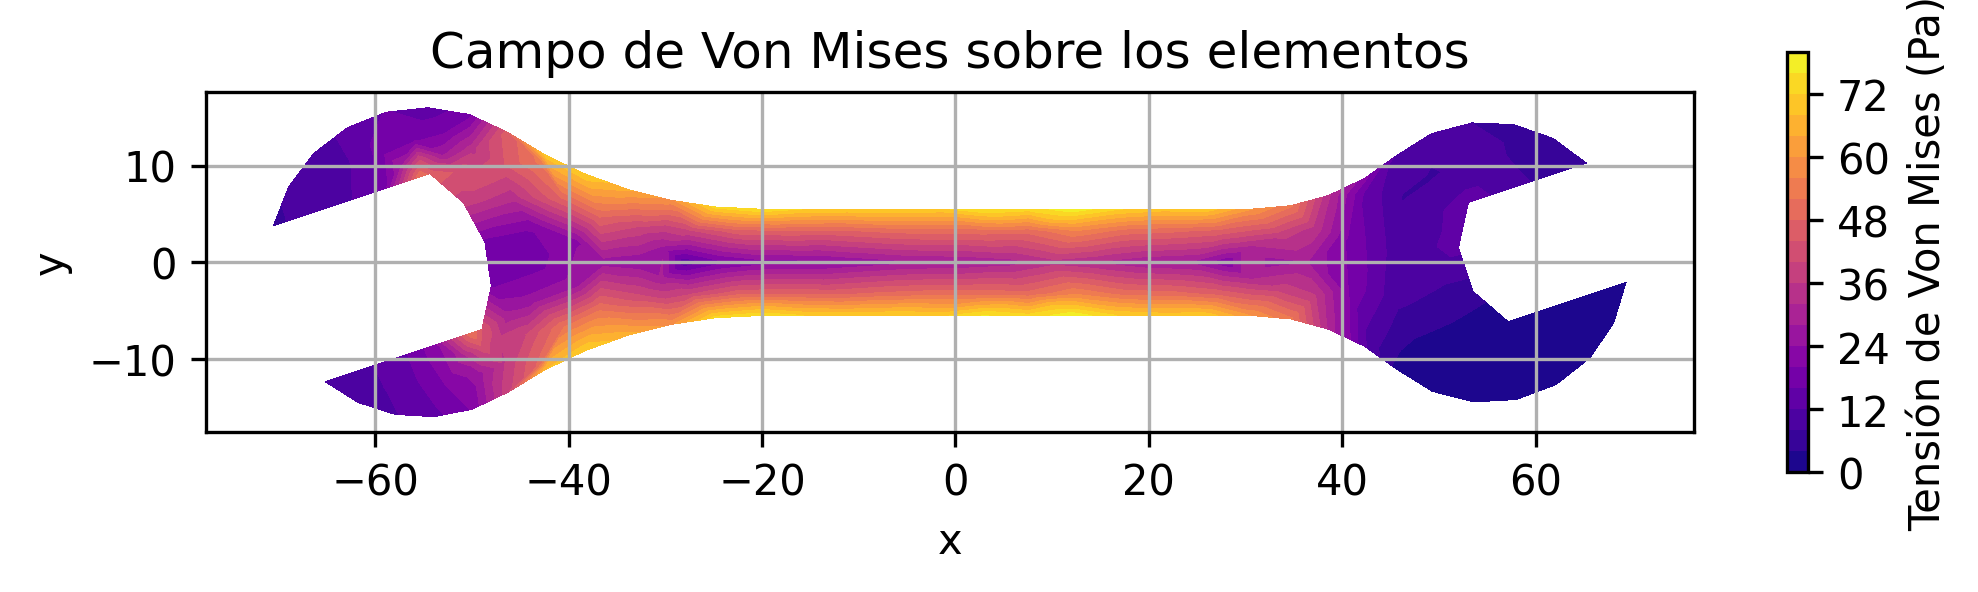
\includegraphics[width=0.8\textwidth]{GRAFICOS/Topo_von_mises.png}
    \caption{Von Mises stress distribution after optimization.}
    \label{fig:von_mises_optimized}
\end{figure}
The optimization process resulted in a more uniform stress distribution, reducing peak stresses and improving the overall performance of the wrench. The final design is expected to be more efficient and durable under mechanical loading conditions.







